\documentclass{beamer}
\usepackage[utf8]{inputenc}
\usepackage[T1]{fontenc}
\usepackage{setspace}
\usepackage{gensymb}
\singlespacing
\usepackage{amsmath}
\usepackage{amssymb}
\usepackage{bm}
\usepackage{cite}
\usepackage{cases}
\usepackage{subfig}
\usepackage{longtable}
\usepackage{multirow}
\usepackage{verbatim}
\usepackage{hyperref}
\usepackage{listings}
\usepackage{xcolor}
\usepackage{array}
\usepackage{calc}
\usepackage{hhline}
\usepackage{ifthen}
\usepackage{textcomp}

\hypersetup{
    colorlinks=true,
    linkcolor=black,
    urlcolor=blue,
}

\usetheme{CambridgeUS}

% Robust listings configuration
\lstset{
    basicstyle=\ttfamily\footnotesize,
    breaklines=true,
    postbreak={\mbox{\textcolor{red}{\tiny$\hookrightarrow$}\space},
    columns=fullflexible,
    keepspaces=true,
    showstringspaces=false,
    upquote=true,
    literate={~}{{\textasciitilde}}1
}

\title[Clock on Vaman FPGA]{Clock Implementation on Vaman FPGA using K-Maps and Multiplexing}
\author{Dhawal Saini\\
}

\begin{document}

\begin{frame}
    \titlepage
    \centering
    Electrical Department\\
    Indian Institute Of Technology, Hyderabad
\end{frame}

\begin{frame}{Outline}
    \tableofcontents
\end{frame}

\section{Introduction}
\begin{frame}{Introduction}
    \begin{itemize}
        \item Digital clock system implemented on Vaman FPGA
        \item Key features:
        \begin{itemize}
            \item Uses Karnaugh maps (K-Maps) for time increment logic
            \item Implements display multiplexing
            \item Single BCD drives six 7-segment displays
        \end{itemize}
        \item Implemented in Verilog HDL
    \end{itemize}
\end{frame}

\section{Components}
\begin{frame}{Components}
    \begin{table}
        \centering
        \begin{tabular}{|l|c|}
        \hline
        \textbf{Component} & \textbf{Quantity}\\
        \hline
        Vaman FPGA Board & 1\\
        \hline
        7-Segment Displays & 6\\
        \hline
        Push Buttons & 4\\
        \hline
        IC 7447 & 1\\
        \hline
        Jumper Wires & 30\\
        \hline
        Breadboards & 2\\
        \hline
        \end{tabular}
    \end{table}
\end{frame}

\section{Circuit Connections}
\begin{frame}{Vaman Connections}
    \begin{columns}
        \begin{column}{0.5\textwidth}
            \begin{itemize}
                \item Button 1: PYGMY 1 (Pause/Play)
                \item Buttons 2-4: PYGMY 2-4 (Time Set)
                \item IC 7447 Inputs: PYGMY 5-8
                \item Display Control: PYGMY 9-14
            \end{itemize}
        \end{column}
        \begin{column}{0.5\textwidth}
            \centering
            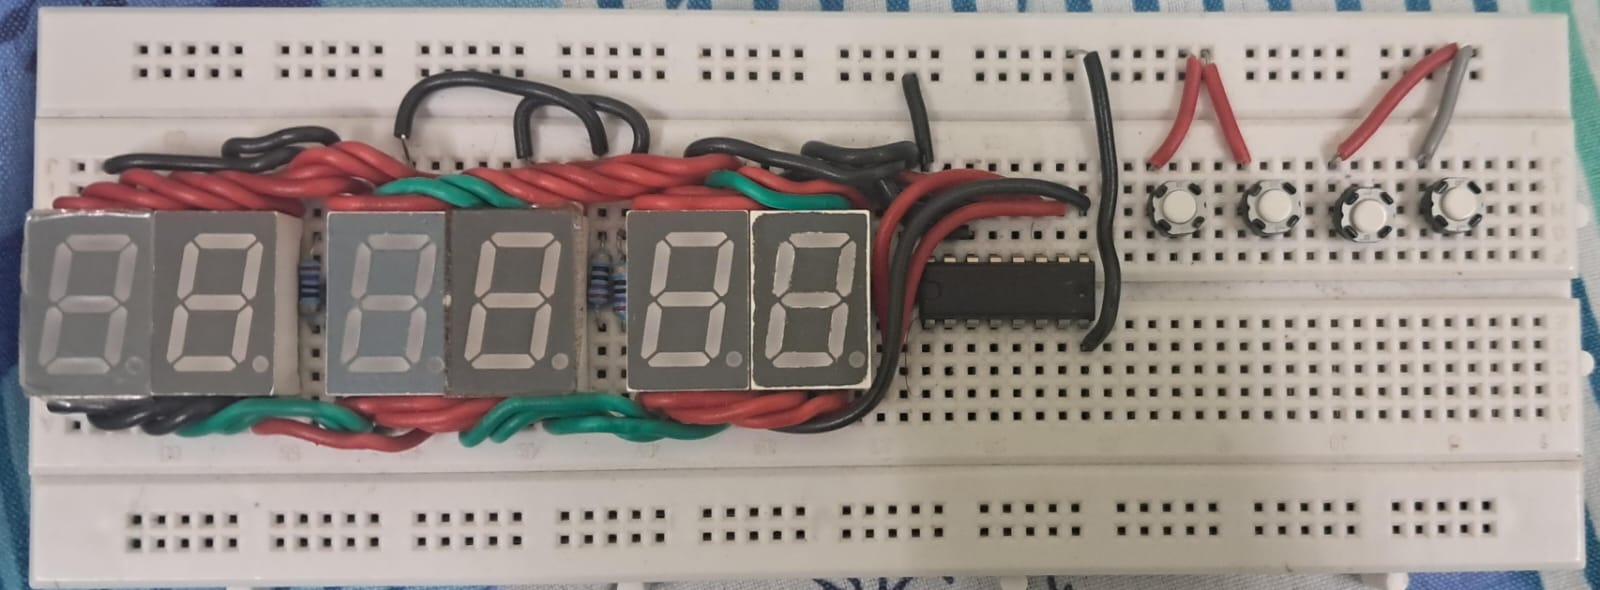
\includegraphics[width=0.9\textwidth]{figs/clock.jpeg}
        \end{column}
    \end{columns}
\end{frame}

\section{Implementation}
\begin{frame}[fragile]{Execution Steps}
    \begin{enumerate}
        \item Clone repository:
        
        \begin{lstlisting}[basicstyle=\ttfamily\small]
git clone https://github.com/ysiddhanth/vaman.git
cd vaman/Clock/codes
        \end{lstlisting}
        
        \item Generate .bin file:
        
        \begin{lstlisting}[basicstyle=\ttfamily\scriptsize]
ql_symbiflow -compile -src . -d ql-eos-s3 -P pu64 -t 
main -v main.v -p quickfeather.pcf
        \end{lstlisting}
        
        \item Program FPGA:
        
        \begin{lstlisting}[basicstyle=\ttfamily\scriptsize]
sudo python3 tinyfpgab --port /dev/ttyACM0 --appfpga main.bin 
--mode fpga --reset
        \end{lstlisting}
    \end{enumerate}
\end{frame}

\section{K-Map Logic}
\begin{frame}{Increment Logic}
    \begin{columns}
        \begin{column}{0.5\textwidth}
            \textbf{Seconds Unit:}
            \begin{align*}
                A_1 &= \overline{W_1} \\
                B_1 &= (W_1 \land \overline{X_1}) \lor (\overline{W_1} \land X_1)
            \end{align*}
        \end{column}
        \begin{column}{0.5\textwidth}
            \textbf{Seconds Tens:}
            \begin{align*}
                A_2 &= \overline{W_2} \\
                B_2 &= (\overline{Y_2} \land W_2) \lor (\overline{W_2} \land X_2)
            \end{align*}
        \end{column}
    \end{columns}
\end{frame}

\section{Conclusion}
\begin{frame}{Summary}
    \begin{itemize}
        \item Successfully implemented digital clock on FPGA
        \item Key achievements:
        \begin{itemize}
            \item Efficient K-Map based logic
            \item Optimized display multiplexing
            \item Flexible control interface
        \end{itemize}
        \item Future enhancements:
        \begin{itemize}
            \item Add date display functionality
            \item Implement alarm features
            \item Optimize power consumption
        \end{itemize}
    \end{itemize}
\end{frame}

\end{document}
